\chapter{Validación y resultados}

\noindent
En esta sección se muestran los resultados obtenidos después de la
implementación. En primer lugar se realizaron un conjunto de pruebas para
validar que el sistema tuviera las propiedades deseadas. Se validó que el último
módulo, la búsqueda en árbol de información perfecta, calculara jugadas con buen
desempeño. Asimismo, se muestra el desempeño del sistema y se contrasta con los
requerimientos y restricciones planteadas al inicio del escrito.

\section{Validación de MCTS}

A lo largo del desarrollo, la metodología de  \textit{Test Driven Development}
fue útil para ganar certidumbre sobre el correcto funcionamiento del programa.
Aun así, contar con pruebas unitarias no asegura que las partes del sistema
funcionen correctamente en conjunto. Después de integrar las reglas de dominó
con MCTS, era necesario validar que el resultado de la búsqueda fuera una jugada
con buen desempeño.

Para verificar que la integración con la librería mctspy era correcta, se
realizaron una serie de simulaciones entre un equipo de jugadores MCTS y un
equipo de jugadores greedy. Cabe resaltar que los jugadores MCTS conocían todas
las fichas, incluyendo las de sus contrincantes. Por otro lado, para los
jugadores greedy es irrelevante conocer las fichas de sus contrincantes, ya que
su jugada se calcula exclusivamente con la información de sus propias fichas.

\begin{figure}[ht]
    \begin{center}
        \hbox{\hspace{-1em} 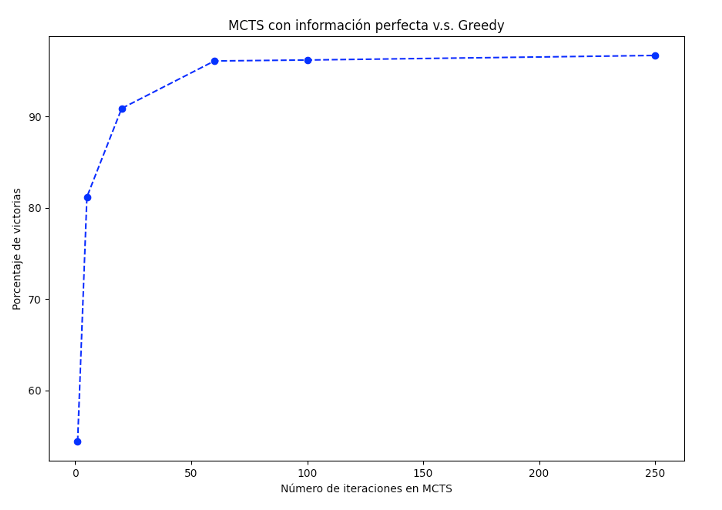
\includegraphics[scale=0.9]{mcts_greedy_abierto.png}}
        \caption{MCTS v.s. Greedy. MCTS vence en más del 90\% de los juegos con 50 simulaciones de MCTS}
        \label{MGA}
    \end{center}
\end{figure}

En la figura \ref{MGA} tenemos una gráfica del resultado de las simulaciones. En
el eje horizontal se muestra el número de iteraciones que se le permitió
ejecutar a MCTS para cada tiro. Se corrieron seis simulaciones con distintas
configuraciones de MCTS de mil juegos cada una. Podemos observar que muy
rápidamente se llega a superar al equipo greedy. Con menos de 20 iteraciones, la
búsqueda en árbol logró vencer al jugador greedy en 80\% de los juegos.

El desempeño observado nos indica que MCTS está calculando buenas jugadas y que
el módulo funciona correctamente.


\section{Desempeño del sistema}

El análisis anterior fue útil para encontrar una combinación de parámetros
adecuada para satisfacer los requerimientos y las restricciones del problema. El
sistema necesita que se definan dos parámetros. El número de iteraciones de
búsqueda y el número de escenarios que se simulan. Ya que el desempeño de MCTS
contra greedy no requería un gran número de iteraciones, se decidió correr
veinte iteraciones de MCTS por cada escenario. Por otro lado, se eligió simular
cien escenarios por tiro.

Se simularon mil juegos de dominó (donde cada jugador sólo conoce sus fichas)
entre el equipo PIMC contra un equipo greedy. El sistema consiguió 74\% de
victorias y el tiempo que tomó en cada tirada fue de 1.2 segundos corriendo en
el servidor de Digital Ocean.